\documentclass[fleqn, a4paper, 12pt]{article}       %fleqn => flushleft equation, setzte alle Formeln linksbündig
\usepackage[ngerman]{babel}
\usepackage[utf8]{inputenc}
\usepackage[official]{eurosym}
\usepackage{amsmath}
\usepackage[onehalfspacing]{setspace}
\usepackage{booktabs}
\usepackage{siunitx}
\sisetup{locale=DE}
\sisetup{per-mode=fraction}
\usepackage{graphicx}
\usepackage{pdfpages}
\usepackage{wrapfig}
\usepackage{subfigure}
\usepackage[toc,page]{appendix}

%Für Zitate
\usepackage[backend=biber,style=alphabetic]{biblatex}   %evtl immer mal wieder <biber Kurzbericht_ELK1_arndt-karger.bcf > laufen lassen; \cite{tl084}

\addbibresource{literatur.bib}


\begin{document}

\begin{titlepage}
	\centering
	%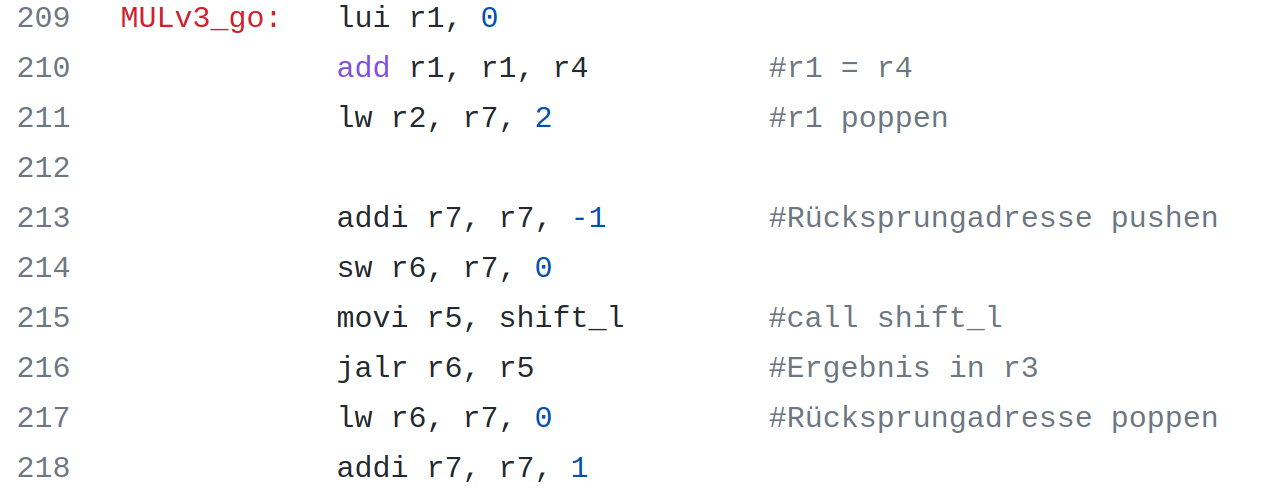
\includegraphics[width=0.8\textwidth]{Titelbild.png}\par\vspace{1cm}
	{\scshape\LARGE Technische Hochschule Mittelhessen \par}
	\vspace{1cm}
	{\huge\bfseries Projektarbeit \par}
	\vspace{1.5cm}
	{\scshape\Large Systemroutinen für RiSC16 Prozessor \par}
	\vspace{2cm}
	{\Large\itshape Arndt Karger\par}
	\vfill
	beleitet durch\par
    Prof. Dr.-Ing. Werner Bonath
	\vfill

% Bottom of the page
	{\large \today\par}
\end{titlepage}

\newpage
\setcounter{page}{0}
\tableofcontents
\newpage


\section{Kurzfassung}
bla

\section{Erstellte Routinen}
\subsection{Stackoperationen}
\subsection{Multiplikation via Addition}
bla
\subsection{Linksschieben via Addition}
bla
\subsection{Bitweise Multiplikation}
bla

\section{Zusammenfassung und Fazit}
bla


\appendix
\thispagestyle{empty}
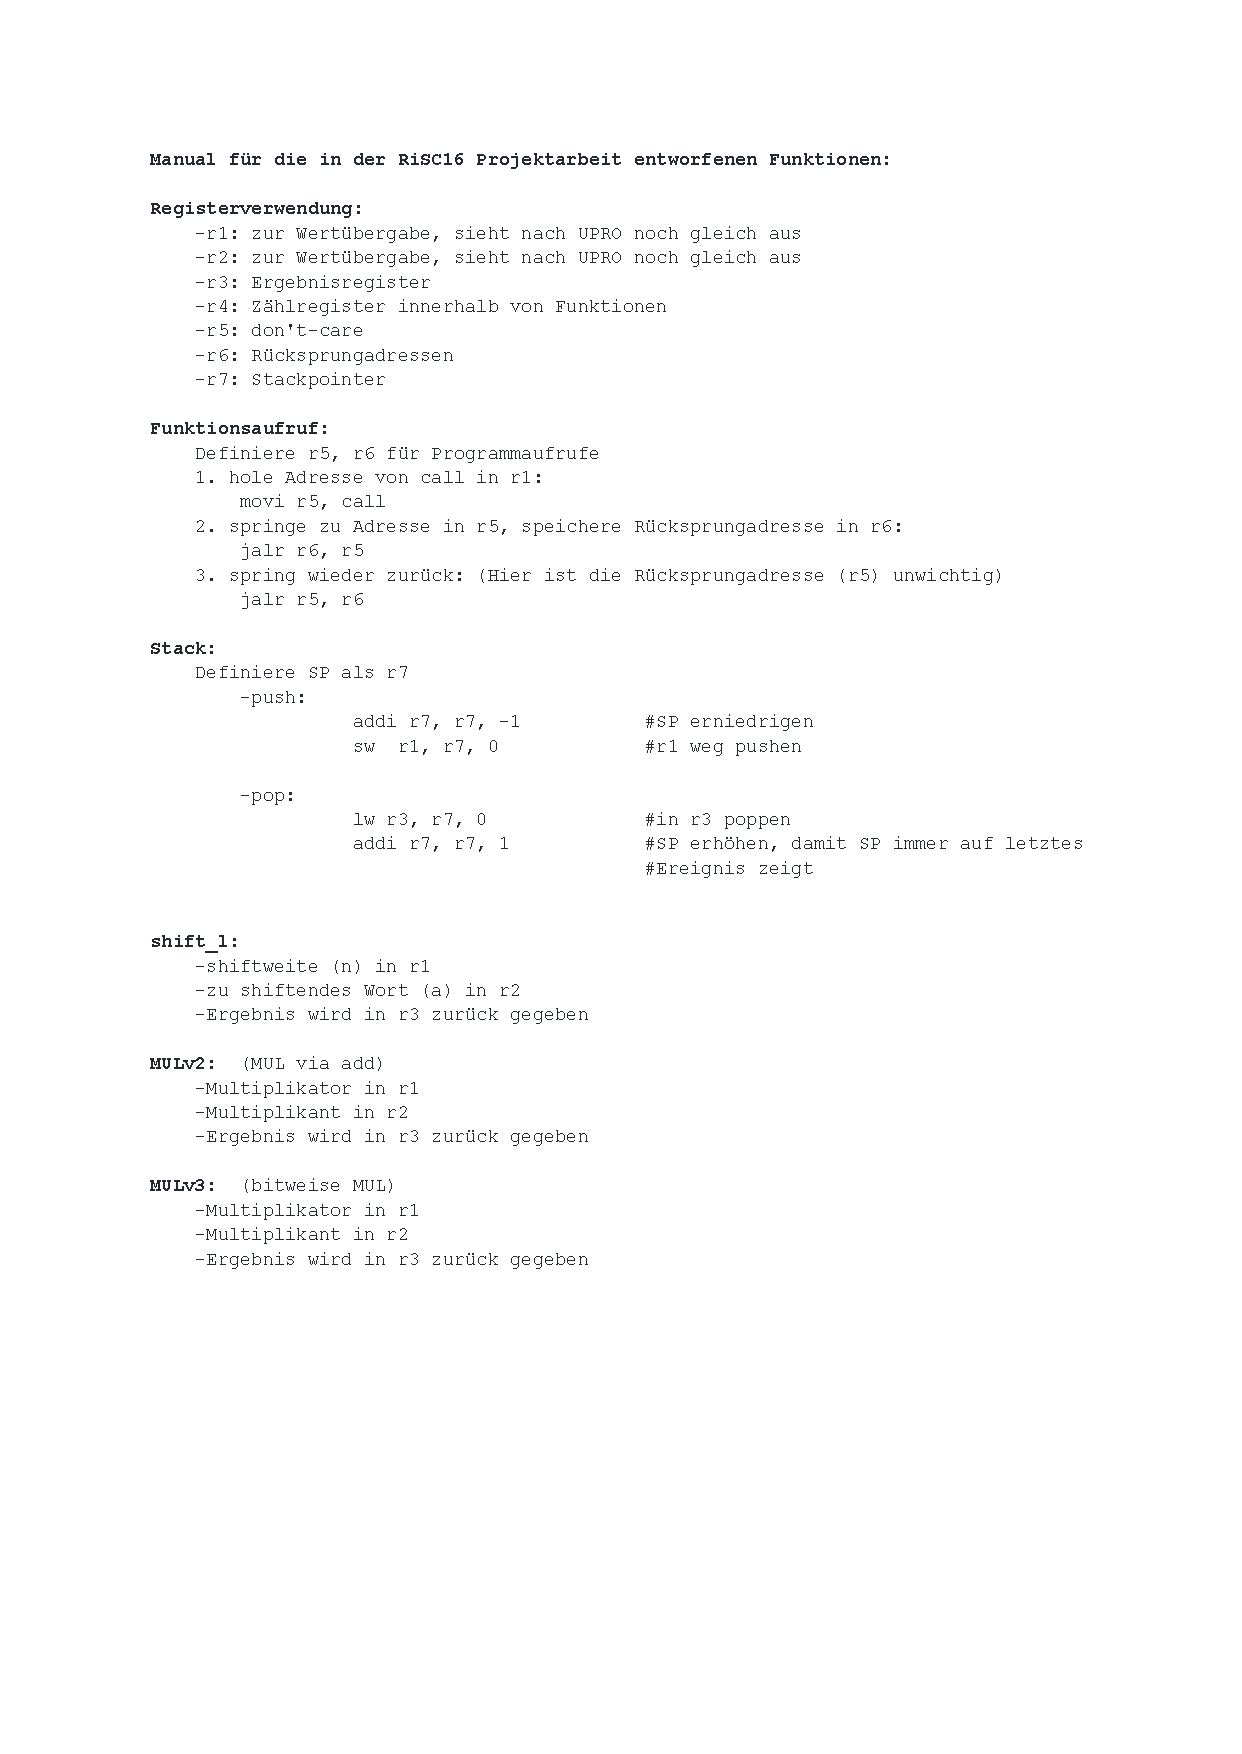
\includepdf[pages=1]{/home/arndt/share_pc_laptop/Uni/thm/Projektarbeit/Dokumentation/Manual.pdf}
\thispagestyle{empty}
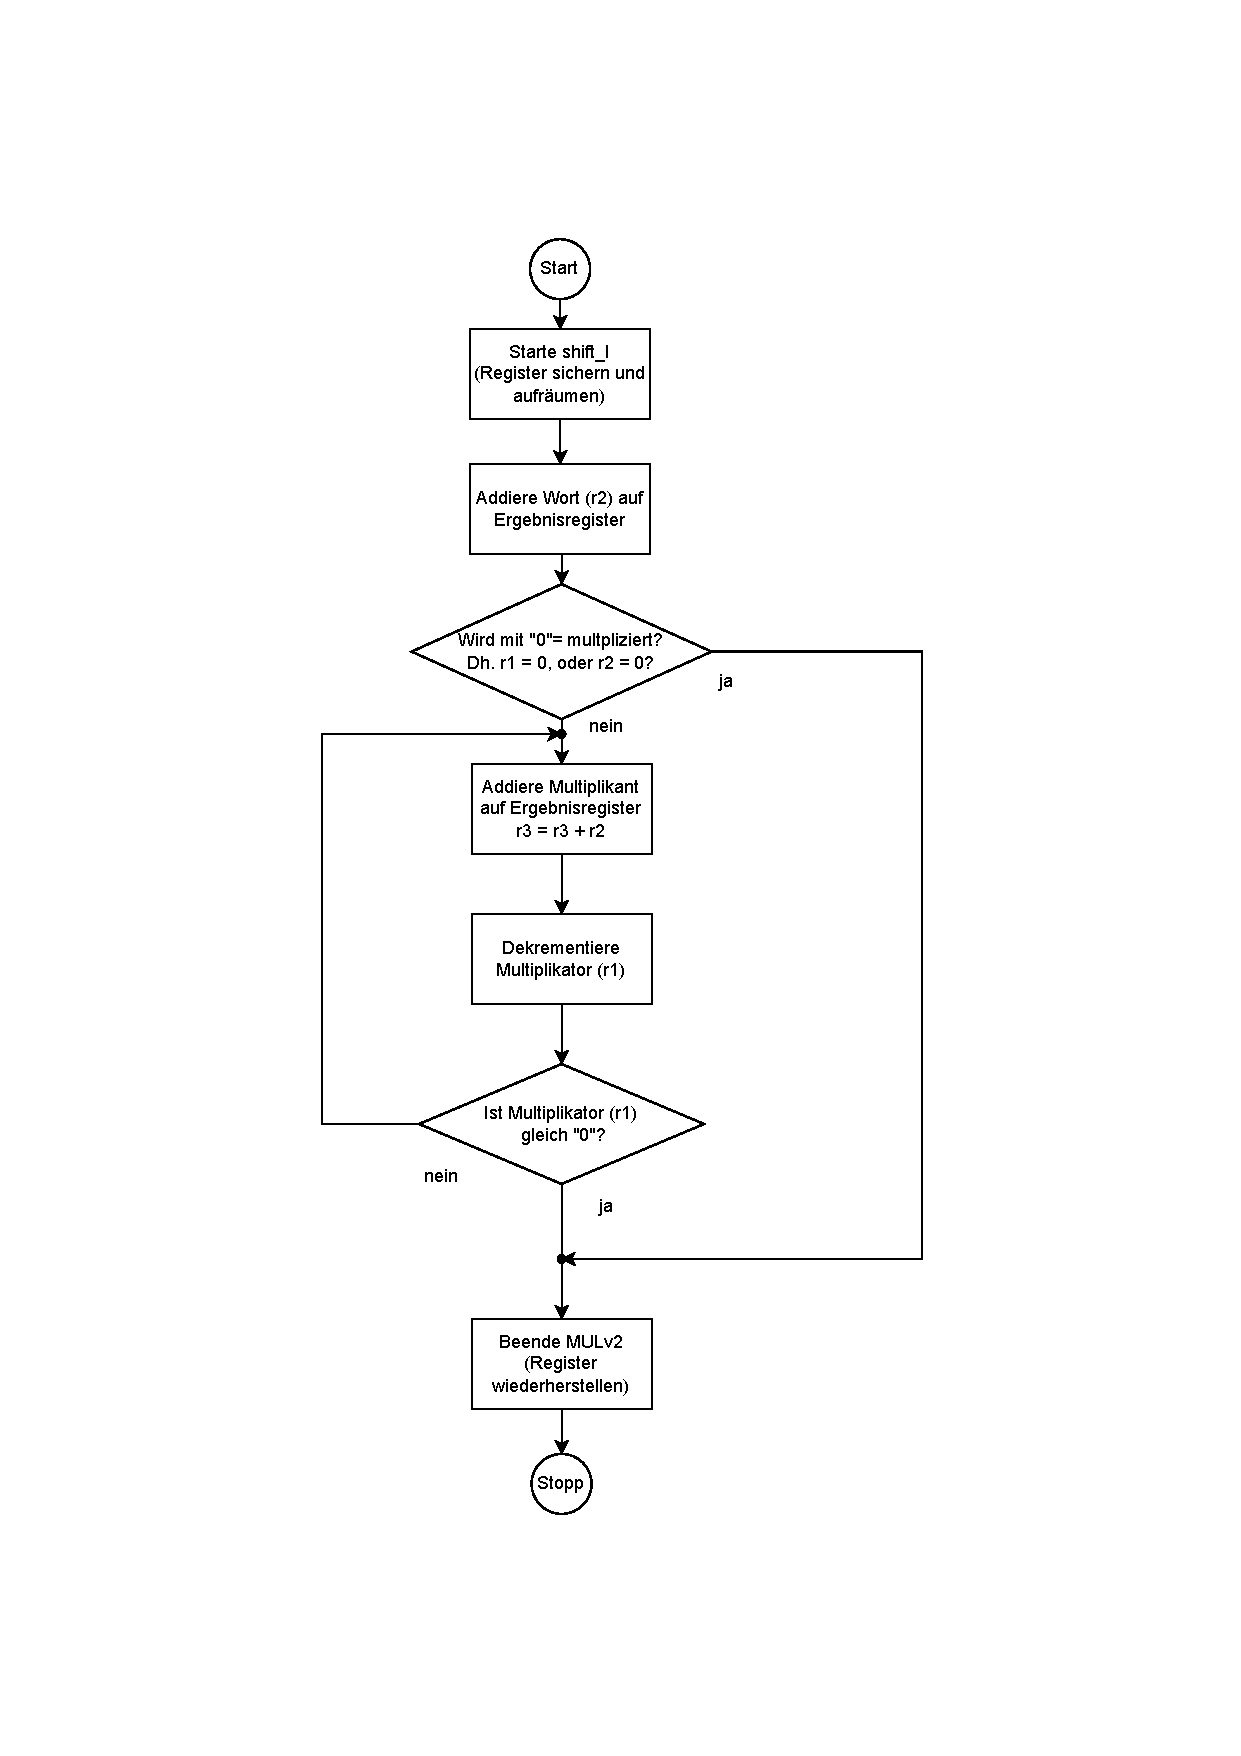
\includepdf[pages=1]{/home/arndt/share_pc_laptop/Uni/thm/Projektarbeit/Dokumentation/MULv2.pdf}

\thispagestyle{empty}
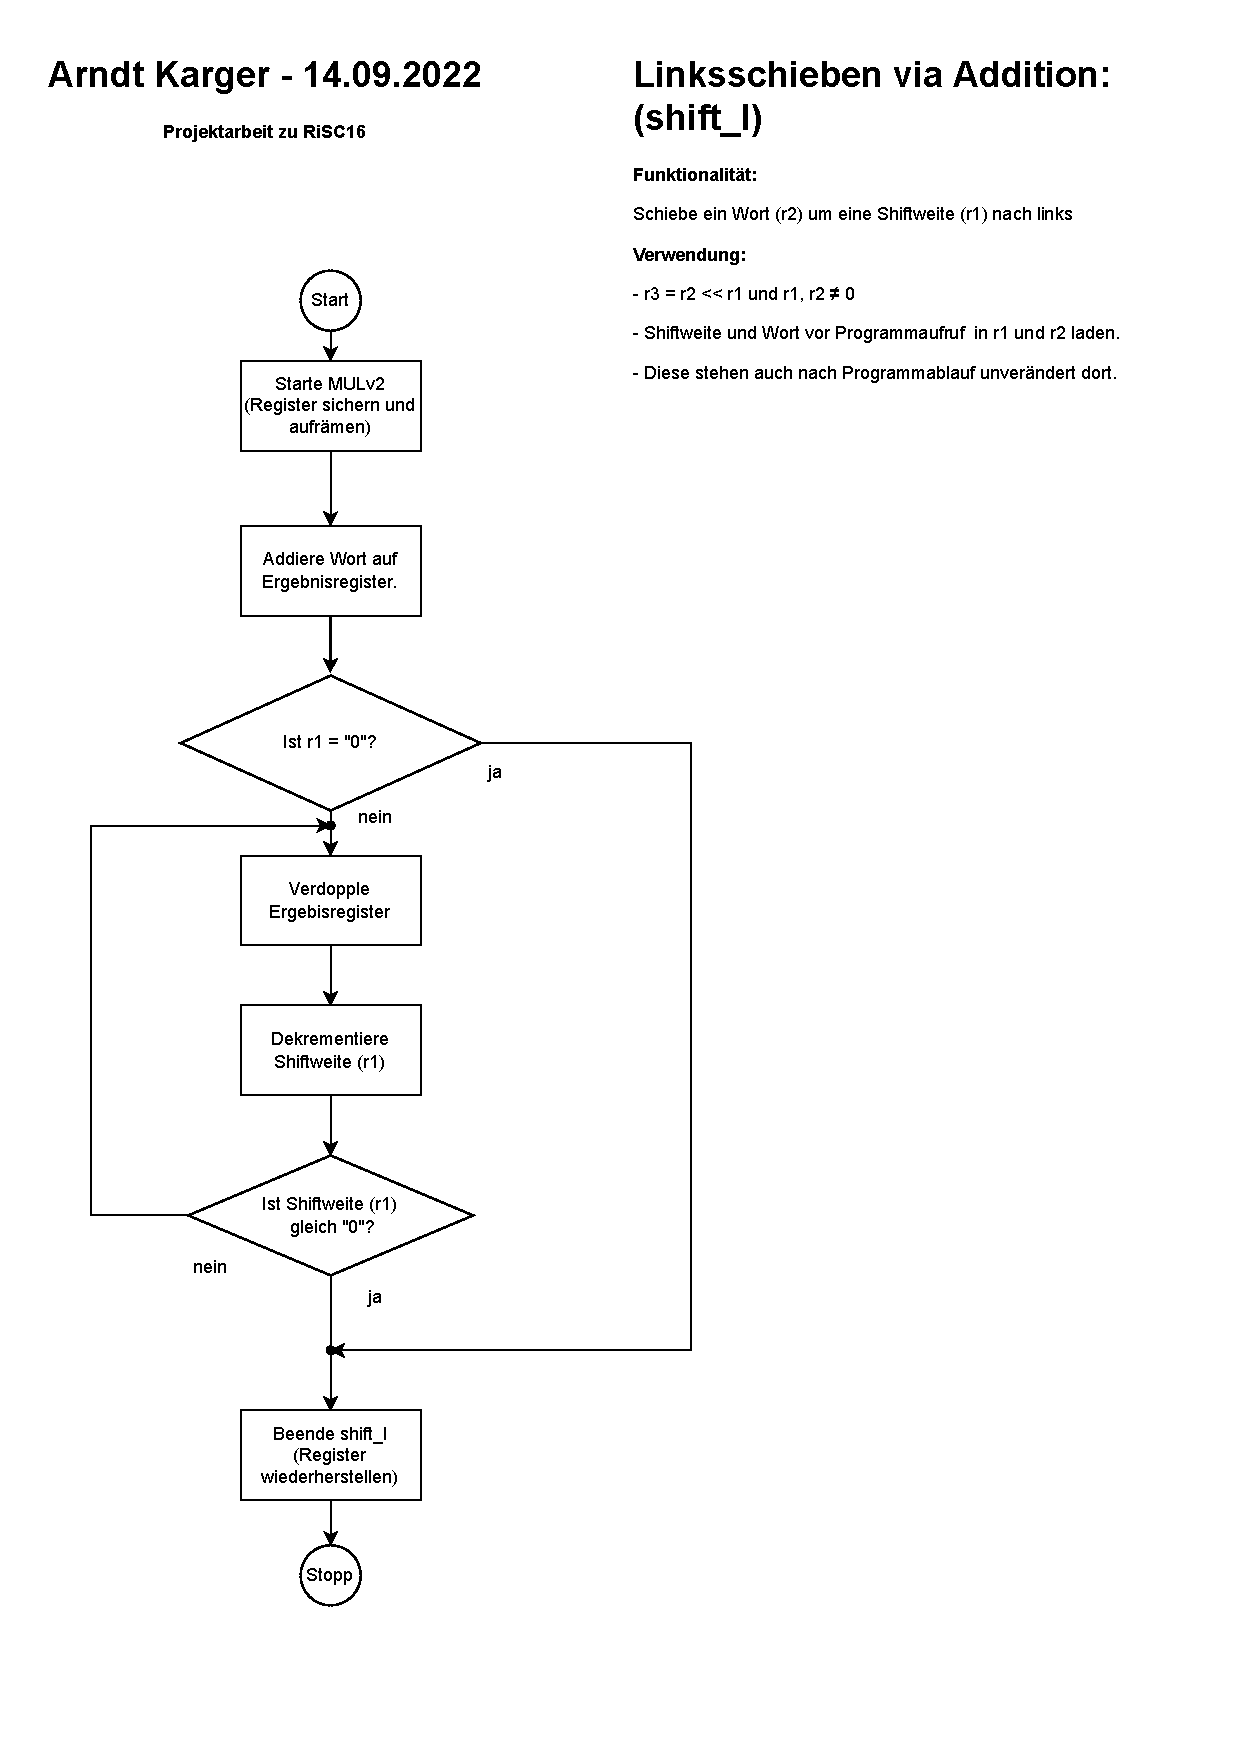
\includepdf[pages=1]{/home/arndt/share_pc_laptop/Uni/thm/Projektarbeit/Dokumentation/shift_l.pdf}

\thispagestyle{empty}
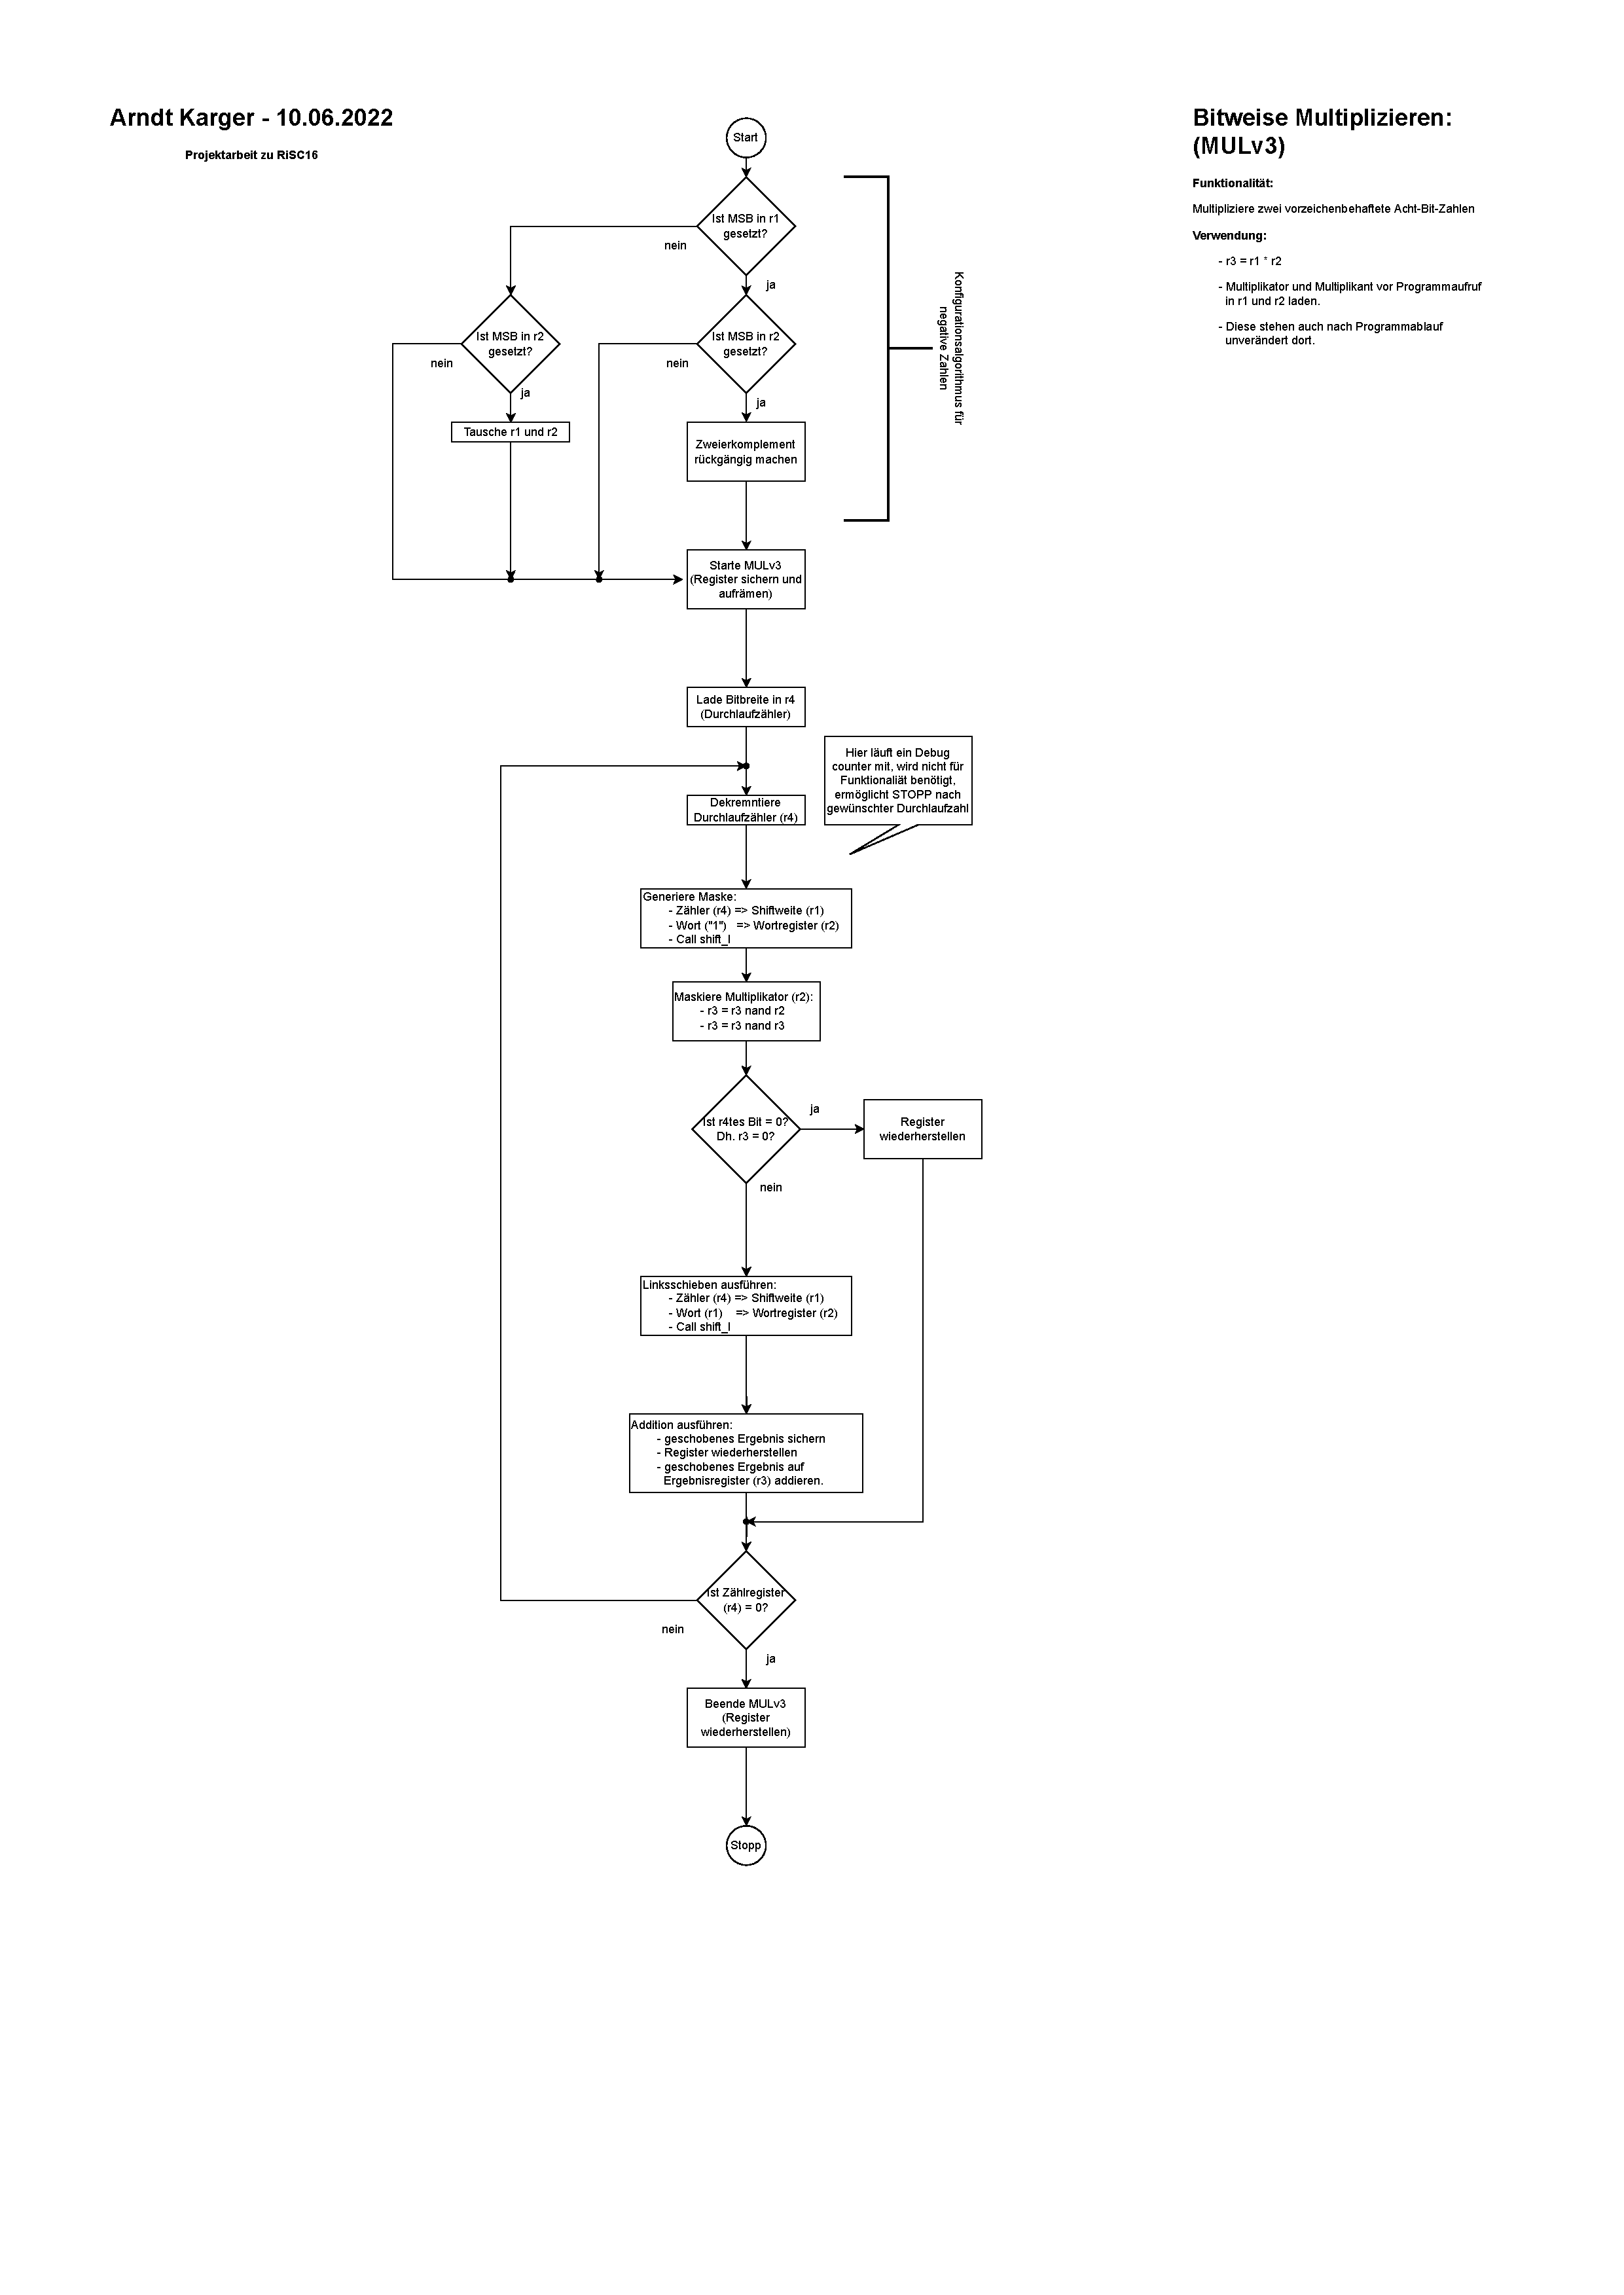
\includepdf[pages=1]{/home/arndt/share_pc_laptop/Uni/thm/Projektarbeit/Dokumentation/MULv3_Flowchart.pdf}

\thispagestyle{empty}
\includepdf[pages=2]{/home/arndt/share_pc_laptop/Uni/thm/Projektarbeit/Dokumentation/MULv3_Flowchart.pdf}



\newpage
\printbibliography  % so werden Zitate angegeben: \cite{name}





















\end{document}

